\section{Theory}
\label{sec:theory}

The solution will be to utilize a Gaussian Mixture Model (GMM) to represent the
inverse kinematics map. My presentation will closely follow three
sources:~\cite{mclachlan2007algorithm,ghahramani1993solving,xu2017data}.

We assume that the data $\Xi = \left\{ \xi_1, \ldots, \xi_N \right\}$ were
generated independently by a mixture density:
%
\begin{equation}
    P(\xi_i) = \sum_{j=1}^M \underbrace{P(\omega_j)}_{\pi_j} 
        P(\xi_i \mid \omega_j; \psi_j),
    \label{eq:mixture_density}
\end{equation}
%
where $\{\pi_j\}_j^M$ are the mixture proportions, each component of the mixture
is denoted $\omega_j$ and parametrized by $\psi_j$. The mixture proportions are
to be picked such that \[ \sum_{j=1}^M \pi_j = 1. \] The full set of parameters
of this model are $\pi_j$'s and $\psi_j$'s. We will write $\Psi = (\pi_j,
\psi_j)_j$. When we restrict these probability distributions to be Gaussian, we
will further have $\psi_j = (\mu_j, \Sigma_j)$, where $\mu_j$ is the mean and
$\Sigma_j$ the covariance of the $j^{\textrm{th}}$ Gaussian. The log of the
likelihood of the parameters given the data set is
%
\begin{equation}
    \ell(\Psi \mid \Xi) = \log{ \prod_{i=1}^N \sum_{j=1}^M P(\xi_i \mid \omega_j; 
    \psi_j) P(\omega_j) } = \sum_{i=1}^N \log{ \sum_{j=1}^M 
    P(\xi_i \mid \omega_j; \psi_j) P(\omega_j). }
    \label{eq:loglike}
\end{equation}
%
We seek to find the parameter vector $\Psi$ that maximizes $\ell(\Psi \mid
\Xi)$. However, this function is not easily maximized numerically because it
involves the log of a sum. Intuitively, it is not easily maximized because for
each data point, there is a ``credit-assignment'' problem, i.e., it is not clear
which component of the mixture generated the data point and thus which
parameters to adjust to fit that data point.

The expectation maximization (EM) algorithm applied to mixtures is an iterative
method for overcoming this credit-assignment problem. The intuition behind it is
that if one had access to a ``hidden'' random variable $z$ that indicated which
data point was generated by which component, then the maximization problem would
decouple into a set of simple maximizations. Mathematically, given $\mc{Z} =
\{z_1, \ldots, z_N \}$ a ``complete-data'' log likelihood function could be
written,
%
\begin{equation}
    \ell_c(\Psi \mid \Xi, \mc{Z}) = \sum_{i=1}^N \sum_{j=1}^M z_{ij} \log{
        P(\xi_i \mid z_i; \Psi)P(z_i; \Psi),
    }
    \label{eq:complete_loglike}
\end{equation}
%
such that it does not involve a log of a summation.

As proven in~\cite{dempster1977maximum}, $\ell(\Psi \mid \Xi)$ can be maximized
by iterating the following two steps,
%
\begin{align}
    \begin{split}
    \text{E-step: } \quad &Q(\Psi \mid \Psi_k) = \mathbb{E}\left[ \ell_c(\Psi \mid \Xi, \mc{Z}) \mid \Xi, \Psi_k \right] \\
    \text{M-step: } \quad &\Psi_{k+1} = \arg \max_\Psi Q(\Psi \mid \Psi_k).
    \end{split}
    \label{eq:EM_alg}
\end{align}
%
The E (Expectation) step computes the expected complete data log likelihood and 
the M (Maximization) step finds the parameters that maximize this likelihood.

\subsection{Mixture of Gaussians}
Let me now specialize to the case where the probability functions above are
Gaussians. For this model, the E-step simplifies to computing $h_{ij} =
\mathbb{E}\left[ z_{ij} \mid \xi_i, \psi_k \right]$, the probability that
Gaussian $j$, as defined by the mean $\hat{\mu}_j$ and covariance matrix
$\hat{\Sigma}_j$ estimated at time step $k$, generated data point $i$:
%
\begin{equation}
    h_{ij}^{(k)} = \frac{\abs{\hat{\Sigma}_j^{(k)}}^{-\frac{1}{2}} 
    \exp{\left\{-\frac{1}{2}\left( \xi_i - \hat{\mu}_j^{(k)} \right)^\top 
    \left({\hat{\Sigma}_j^{(k)}}\right)^{-1} \left( \xi_i - \hat{\mu}_j^{(k)} \right) \right\}}  }
    {\sum_{l=1}^M \abs{\hat{\Sigma}_l^{(k)}}^{-\frac{1}{2}} 
    \exp{\left\{-\frac{1}{2}\left( \xi_i - \hat{\mu}_l^{(k)} \right)^\top 
    \left({\hat{\Sigma}_l^{(k)}}\right)^{-1} \left( \xi_i - \hat{\mu}_l^{(k)} \right) \right\}} }.
    \label{eq:E-step}
\end{equation}
%
The M-step then involves re-estimating the means and covariances of the
Gaussians along with the mixing proportions using the data set weighted by the
$h_{ij}$:
%
\begin{align}
    \begin{split}
    \hat{\mu}_j^{(k+1)} &= \frac{\sum_{i=1}^N h_{ij}^{(k)}\xi_i}{\sum_{i=1}^N h_{ij}^{(k)}}, \\
    \hat{\Sigma}_j^{(k+1)} &= \frac{\sum_{i=1}^N h_{ij}^{(k)} \left(\xi_i - \hat{\mu}_j^{(k+1)}\right)
                    \left(\xi_i - \hat{\mu}_j^{(k+1)}\right)^\top}{\sum_{i=1}^N h_{ij}^{(k)}}, \\
    \pi_j^{(k+1)} &= \frac{1}{N}\sum_{i=1}^N h_{ij}^{(k)}.
    \end{split}
    \label{eq:M-step}
\end{align}


\subsection{Supervised Learning}
%
When viewed as supervised learning, each vector $\xi_i$ in the training set is
composed of an ``input'' subvector $\mathrm{x}_i$ and a ``target'' or output
subvector $\theta_i$. Applying the learning algorithm, we obtain an estimate of
the density of the data in this input/output space. This estimate can be used to
approximate a function in the following way:

Given the input vector $\mathrm{x}_i$, we extract all the relevant information
from the joint probability density function (pdf) $P(\mathrm{x}, \theta)$ by
conditionalizing to $P(\theta \mid \mathrm{x})$. For a single Gaussian this
conditional density is normal, and by linearity, since $P(\mathrm{x}, \theta)$
is a mixture of Gaussians, so is $P(\theta \mid \mathrm{x})$. Let me elaborate
on how to compute this posterior (conditional) density for Gaussian mixture
models. First, we partition the mean vector $\hat{\mu}_j$ and the covariance
matrix $\hat{\Sigma}_j$.
%
\begin{equation}
    \hat{\mu}_j = \bmat{\hat{\mu}_{\mathrm{x},j} & \hat{\mu}_{\theta,j}}, \qquad
    \hat{\Sigma}_j = \bmat{
        \Sigma_{\mathrm{xx}, j} & \Sigma_{\mathrm{x}\theta, j} \\
        \Sigma_{\theta\mathrm{x}, j} & \Sigma_{\theta\theta, j}
    }.
    \label{eq:partition}
\end{equation}
%
Given each component $\omega_j$ and output $x$, the conditionial probability 
distributioin of $\theta$ can be obtained as:
%
\begin{align}
    \begin{split}
    P(\theta \mid \mathrm{x}; \omega_j) &= \mc{N}\left( \theta \mid \tilde{\mu}_{\theta,j}, \tilde{\Sigma}_{\theta\theta} \right), \\
    \tilde{\mu}_{\theta, j} &=  \mu_{\theta, j} + \Sigma_{\theta\mathrm{x}, j}\Sigma_{\mathrm{xx}, j}^{-1} \left( \mathrm{x} - \mu_{\mathrm{x},j} \right), \\
    \tilde{\Sigma}_{\theta\theta, j} &= \Sigma_{\theta\theta, j} - \Sigma_{\theta\mathrm{x}, j}\Sigma_{\mathrm{xx}, j}^{-1}\Sigma_{\mathrm{x}\theta, j}.
    \end{split}
    \label{eq:posterior_each_comp}
\end{align}
%
Finally, we marginalize out the component $\omega_j$ to find the conditional 
probability of $\theta$ given $\mathrm{x}$:
%
\begin{align}
    \begin{split}
    P(\theta \mid \mathrm{x}) &= \sum_{j=1}^M \beta_j \mc{N}\left(\theta \mid \tilde{\mu}_{\theta,j}, \tilde{\Sigma}_{\theta\theta,j} \right), \\
    \beta_j &= \frac{\pi_j P(\mathrm{x}_j)}{\sum_{j=1}^M \pi_j P(\mathrm{x}_j)} = 
    \frac{\pi_j \mc{N}\left(\mathrm{x} \mid {\mu}_{\mathrm{x},j}, {\Sigma}_{\mathrm{xx},j} \right)}
    {\sum_{j=1}^M \pi_j \mc{N}\left(\mathrm{x} \mid {\mu}_{\mathrm{x},j}, {\Sigma}_{\mathrm{xx},j} \right)}.
    \end{split}
    \label{eq:posterior_distribution}
\end{align}
%
Here, notice that, to compute $\beta_j$, we compute the probability of observing
the data point $\mathrm{x}$ under the Gaussian distribution whose mean is
$\mu_{\mathrm{x},j}$ and whose covariance is $\Sigma_{\mathrm{xx},j}$, for each
$j$.


In principle, this conditional density is the final output of the density
estimator. That is, given a particular input, the network returns the complete
conditional density of the output. However, for the purposes of comparison to
function approximation methods and since many applications require a single
estimate of the output, I will outline two possible ways to obtain such an
estimate $\hat{\theta}$ of $\theta = f(x)$.

\begin{enumerate}
    \item Stochastic Sampling (STOCH) samples according to the distribution
    $\hat{\theta}(\mathrm{x}) \sim P(\theta \mid \mathrm{x})$:
    %
    \begin{equation*}
        \hat{\theta} = \sum_{j=1}^M \beta_j \tilde{\mu}_{\theta,j}, \qquad
        \hat{\Sigma}_{\theta\theta} = \sum_{j=1}^M \beta_j^2 \tilde{\Sigma}_{\theta\theta,j}.
    \end{equation*}
    %
    \item Single component least-squares estimation (SLSE) takes
    $\hat{\theta}(\mathrm{x}) = \mathbb{E}\left( \theta \mid \mathrm{x},
    \omega_j \right)$, where $j = \arg \max_k (\beta_k \mid \mathrm{x}) = \arg
    \max_k \mc{N}\left(\mathrm{x} \mid \mu_{\mathrm{x},k},
    \Sigma_{\mathrm{xx}_k}\right)$. That is, for a given input, SLSE picks the
    Gaussian with the highest posterior, and for that Gaussian approximates the
    output with the least-squares estimator given by that Gaussian alone.
\end{enumerate}


\subsection{Initialization of Expectation Maximization}
\label{ssec:initialization}
%
The EM algorithm is iterative, which means, in particular, that we need to start
it off with an initial guess for the parameters. Clearly, the better the initial
guess, the faster/easier the convergence will be. The initial guesses I used
were as follows:
%
\begin{enumerate}
    \setlength\itemsep{0.0em}
    \item For $\pi_j$, I used a uniform distribution: $\pi_j^{(0)} =
    \frac{1}{M}$ for all $j = 1, \ldots, M$.
    \item For each $j$, I started the covariance matrix as a multiple of the
    identity matrix: $\Sigma_j^{(0)} = \alpha_j I$.
    \item I used the $k$-means clustering method to generate initial values for
    $\mu_j^{(0)}$. This method aims to partition the $N$ observations into $M
    \leq N$ sets so as to minimize the within-cluster sum-of-squares
    cost~\cite{wiki:K-means_clustering}.
\end{enumerate}
%
\begin{wrapfigure}{r}{0.5\textwidth}
    \vspace{-20mm}
	\centering
	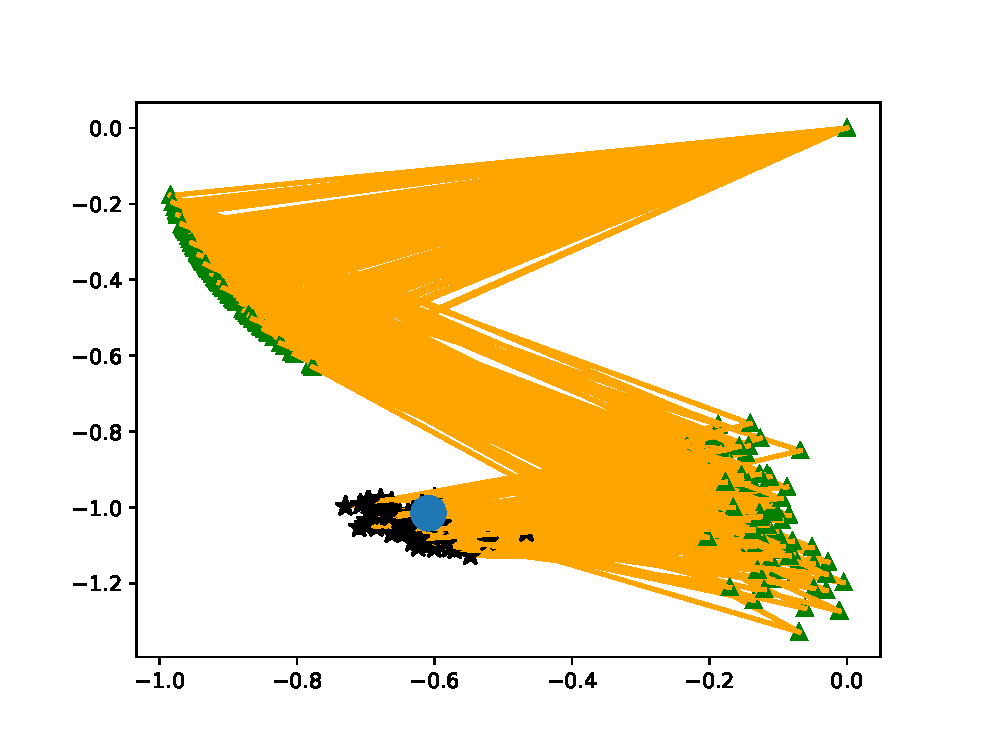
\includegraphics[width=0.5\textwidth]{./figures/GMM_sample_solution.eps}
	\caption{A visualization of the algorithm run with $N=2001$, $M=101$ over
    the range $-\pi \leq \theta_1, \theta_2, \theta_3 \leq \pi$. The desired end-effector position, $\mathrm{x} = \bmat{1.5 &
    -0.4}$, is depicted by the big blue circle. The learned posterior
    distribution $P(\theta \mid \mathrm{x})$ is used to sample $100$ solutions,
    which yield the configurations shown in orange. The actual location of the
    end-effector the orange configurations yield are depicted by the black
    stars.}
    \label{fig:example_sol}
    \vspace{-30mm}
\end{wrapfigure}
%

\subsection{Summary of the Algorithm}
%
Let me provide a brief run-down of the method.

\begin{enumerate}
    \setlength\itemsep{0em}
    \item Randomly select the data points $\{\theta_1, \ldots, \theta_N\}$ and
    generate the corresponding $\{\mathrm{x}_1, \ldots, \mathrm{x}_N\}$.
    %
    \item Collect the full data in one vector: $\xi_i = \bmat{ \mathrm{x}_i,
    \theta_i}$ and $\xi = \{\xi_i\}_{i=1}^N$.
    %
    \item Model the data to be generated independently by a Gaussian mixture
    density~\eqref{eq:mixture_density} and initialize the parameters of the
    model following Section~\ref{ssec:initialization}.
    %
    \item Employ EM to find $P(\xi) = P(\mathrm{x}, \theta)$ using
    equations~\eqref{eq:E-step} and~\eqref{eq:M-step}.
    %
    \item Marginalize the sum of the Gaussians to find $P(\theta \mid
    \mathrm{x})$ using
    equation~\eqref{eq:partition}--\eqref{eq:posterior_distribution}.
    %
    \item Given an end-effector position $\mathrm{x}$, estimate the joint angles
    using STOCH or SLSE.
\end{enumerate}